%%%%%%%%%%%%%%%%%%%%%%%%%%%%%%%%%%%%%%%%%%%%%%%%%%%%%%%%%%%%%%%%%%%%%%%%%%%%%%%%
\section{Simulations}
% \subsection{Anti-Aliasing Filter}
\subsection{MOSFET Gate Driver} \label{apx:sim_mosfet}
Using LTSpice the chosen MOSFET for the \'Cuk Converter hardware implementation was modelled to determine the theoretical maximum current draw for the \SI{100}{kHz} switching frequency. The circuit shown in figure \ref{fig:sim_mosfet_circuit}.
\begin{figure}[H]
    \centering
    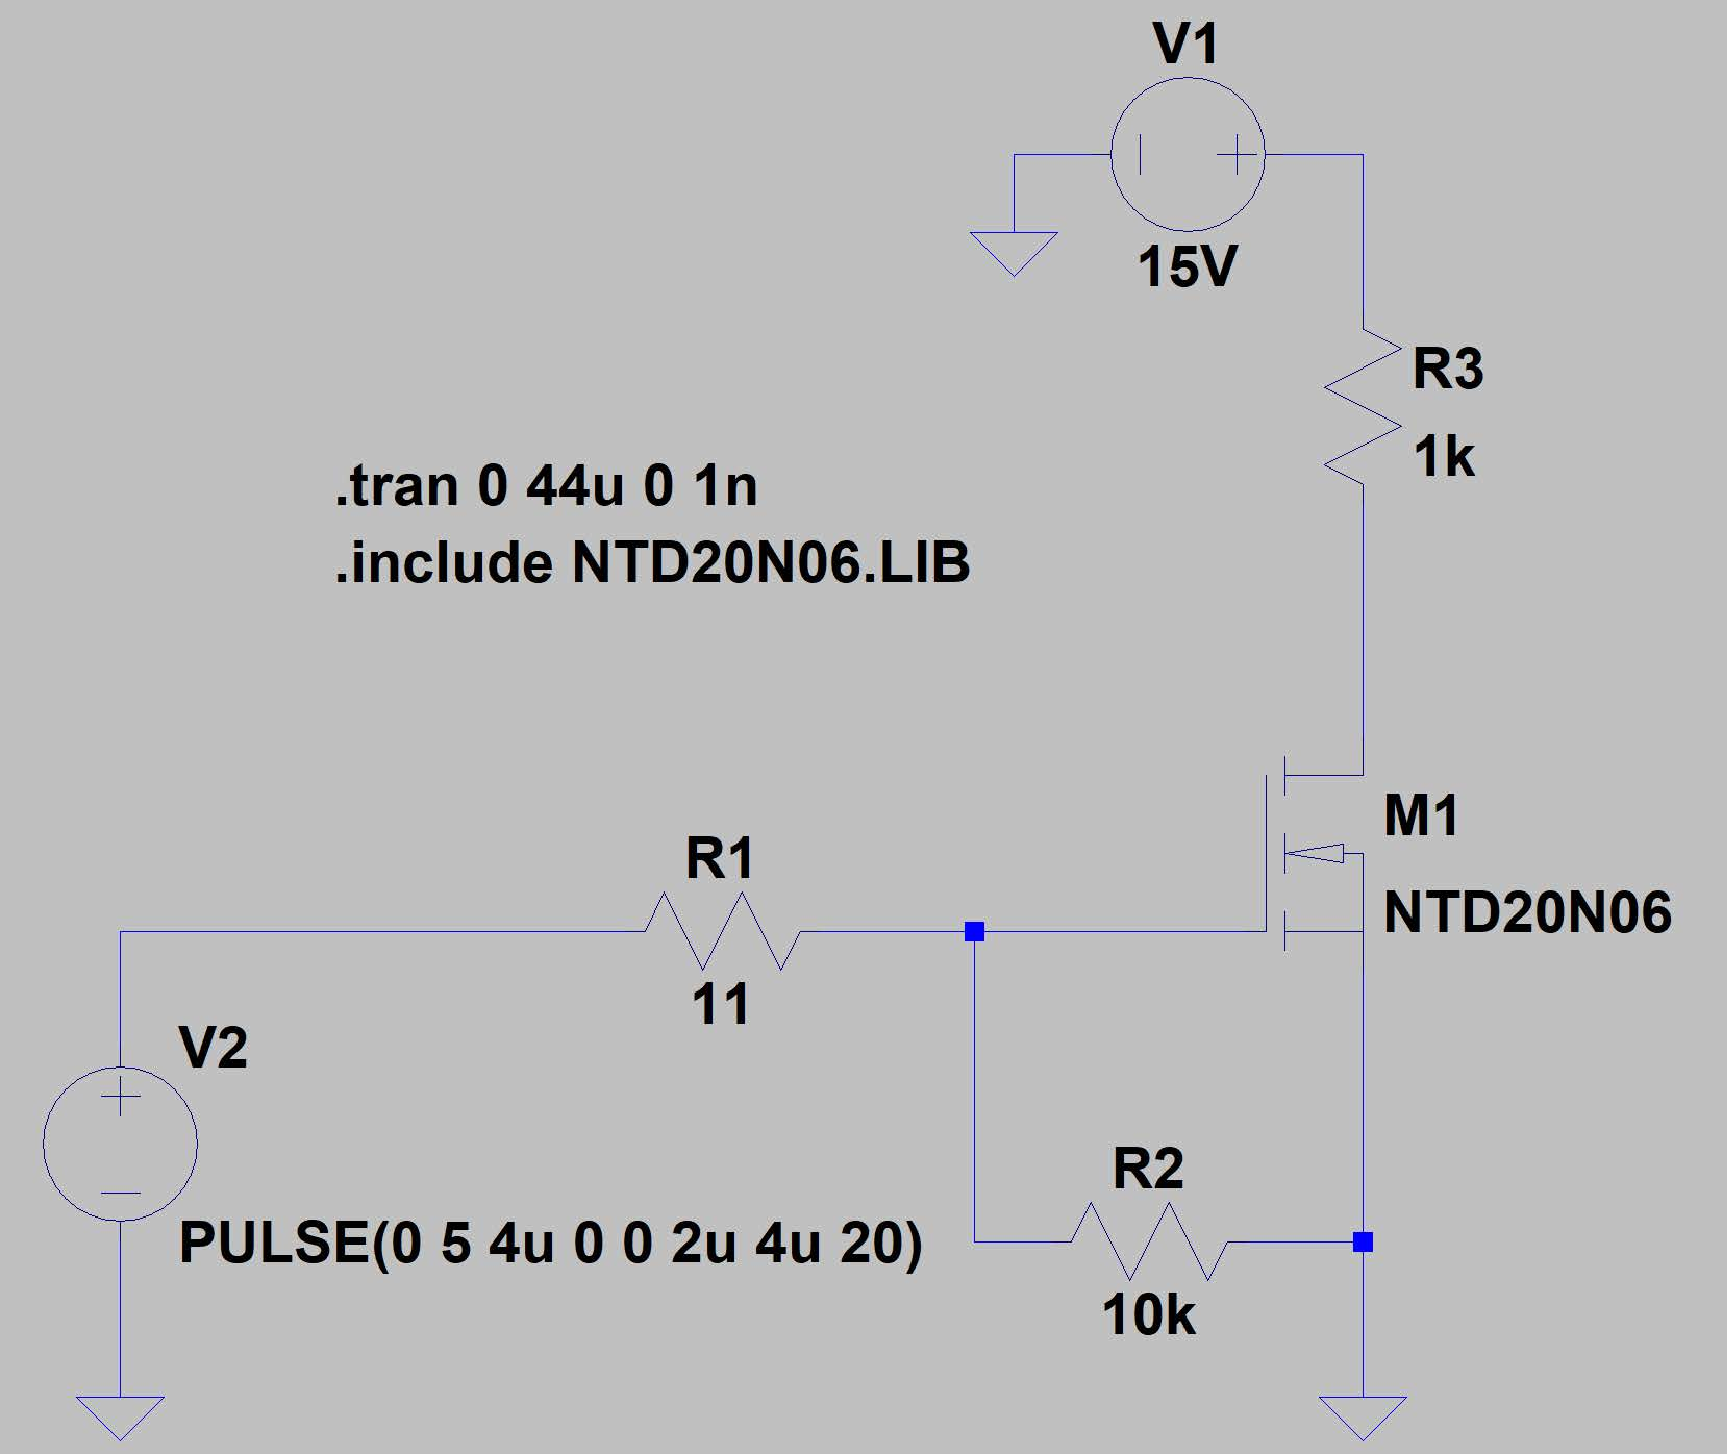
\includegraphics[width = \textwidth]{figures/appendix/sim_mosfet_gate.pdf}
    \caption{MOSFET gate driver simulation circuit.}
    \label{fig:sim_mosfet_circuit}
\end{figure}
Through experimentation the current limiting resistance $R_1$ was varied and found that \SI{10}{\ohm} gave a good compromise between switching speed and current. Despite this the gate current can reach $\pm\SI{180}{mA}$ which well exceeds the input/output source/sink of the microcontroller. This is shown in figure \ref{fig:sim_mosfet_plot}.
\begin{figure}[H]
    \centering
    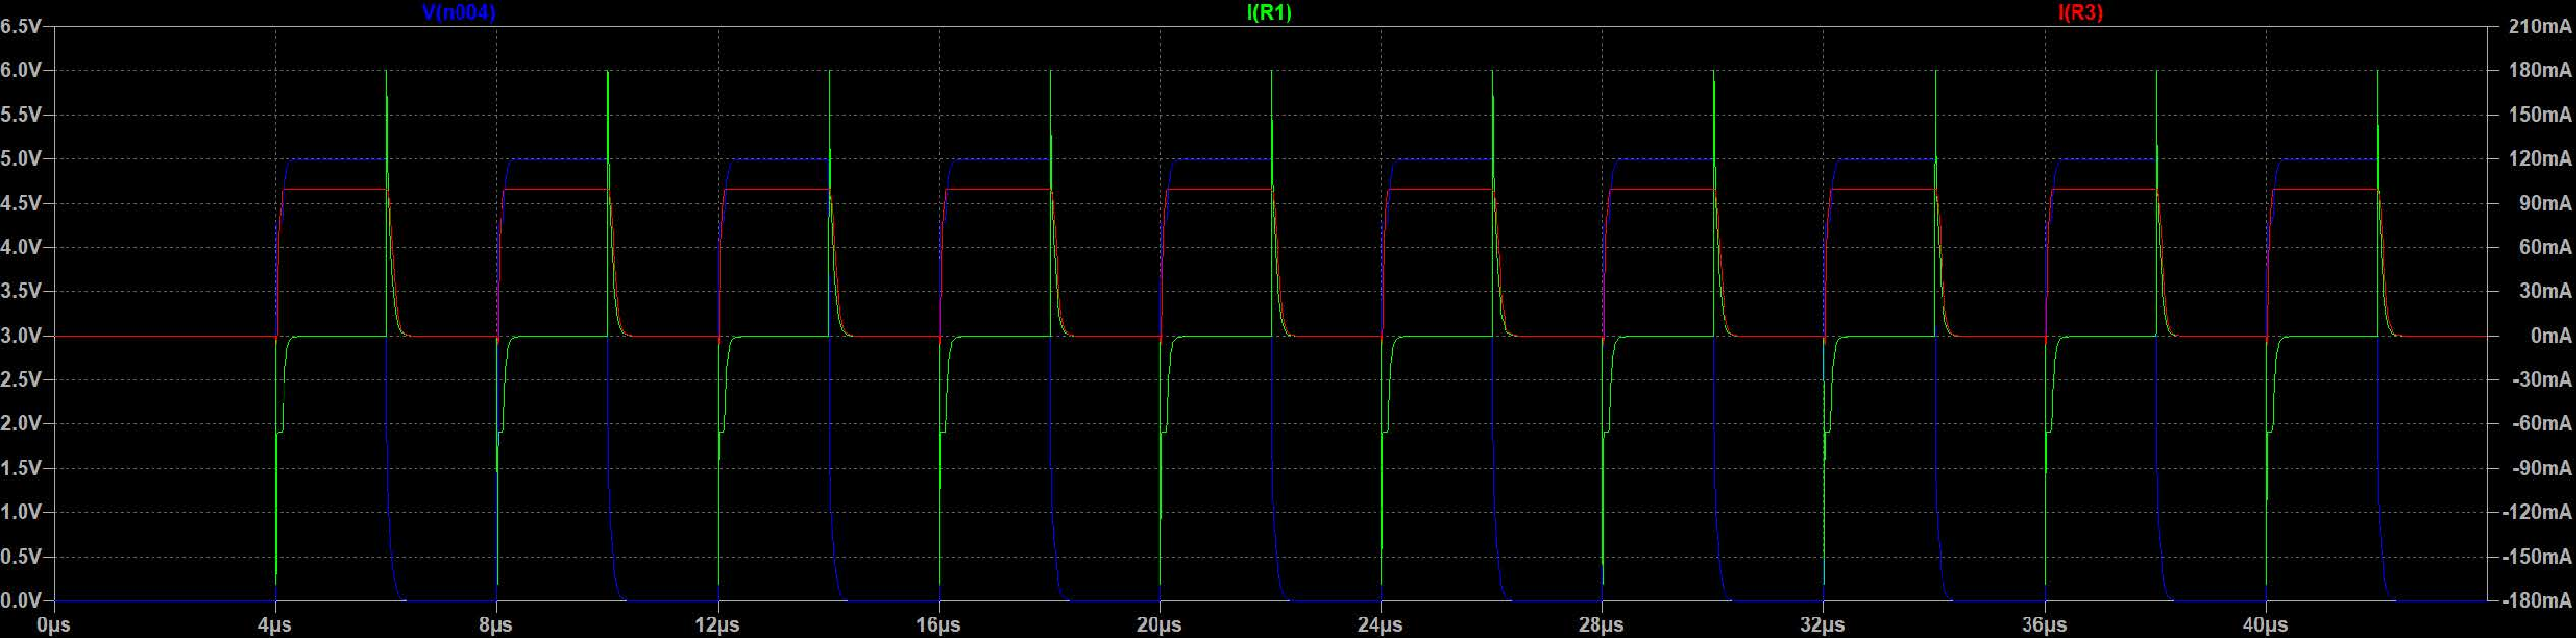
\includegraphics[width = \textwidth]{figures/appendix/sim_mosfet_gate_plot.pdf}
    \caption{MOSFET gate driver simulation plot.}
    \label{fig:sim_mosfet_plot}
\end{figure}
\subsection{\textsf{MATLAB} script}\label{apx:MATLAB}
Used in conjunction with the \textsf{Simulink} model of Figure~\ref{fig:simulink}.
\lstinputlisting{script_MATLAB.m}
%%%%%%%%%%%%%%%%%%%%%%%%%%%%%%%%%%%%%%%%%%%%%%%%%%%%%%%%%%%%%%%%%%%%%%%%%%%%%%%%